\documentclass[11pt,a4paper]{article}
\usepackage[margin=2.2cm]{geometry}
\usepackage{graphicx}
\usepackage{enumitem}
\usepackage{xcolor}
\usepackage[colorlinks=true,linkcolor=blue!50!black,urlcolor=blue!50!black]{hyperref}
\usepackage{parskip}
\setlist[itemize]{leftmargin=1.4em,itemsep=2pt,topsep=3pt}
\newcommand{\decide}[1]{\textcolor{red!75!black}{\textbf{[DECISION: #1]}}}

\title{\vspace{-1.5cm}Tree mortality and ecosystem functional properties\\[2pt]
\large Working draft for coauthors --- bullet points and figures only}
\author{}
\date{\today}

\begin{document}
\maketitle
\vspace{-1cm}

\section*{Scope of this draft}
\begin{itemize}
  \item \textbf{Dataset:} tree cover $\geq$30\,\% within a 500\,m buffer --- \textbf{93 sites, 395 site-years}.
        The unfiltered network (112 sites) and a stricter $\geq$50\,\% subset (65 sites) exist and are held
        for the supplement.
  \item \textbf{Models shown:} \textbf{M3 (climate + traits)} vs \textbf{M4 (climate + traits + disturbance)} only.
        The pair differs solely by the disturbance block, so it isolates its contribution.
  \item \textbf{Learners:} Random forest, XGBoost and LightGBM, \textbf{all tuned with Optuna} (TPE, 50 trials
        per response, grouped 5-fold CV on disjoint site groups).
  \item \textbf{Windows:} 12-month and 24-month climate aggregation, both shown.
  \item \textbf{Cross-validation:} leave-one-site-out \emph{and} repeated leave-one-site-out
        (3 $\times$ 80\,\% of sites), both shown.
  \item \textbf{Responses:} GPP$_{sat}$, NEP$_{max}$, ET$_{max}$, WUE. \textbf{uWUE is dropped} from this version.
  \item Everything is filtered from results already computed; no models were retrained.
\end{itemize}

\section*{Figure 1 --- Sites and EFP distributions}
\begin{itemize}
  \item 93 sites: ENF 45, DBF 26, WET 10, MF 6, CSH 2, OSH 2, EBF 1, WSA 1. Median 4 years per site, 2019--2025.
  \item Violins cover all 600 site-years with a valid EFP; modelling uses the 395 with complete predictor coverage.
  \item Between-site variation dominates within-site variation --- which is what leave-one-site-out tests.
  \item \decide{keep all five EFPs in this figure, or drop uWUE here too for consistency?}
\end{itemize}
\begin{center}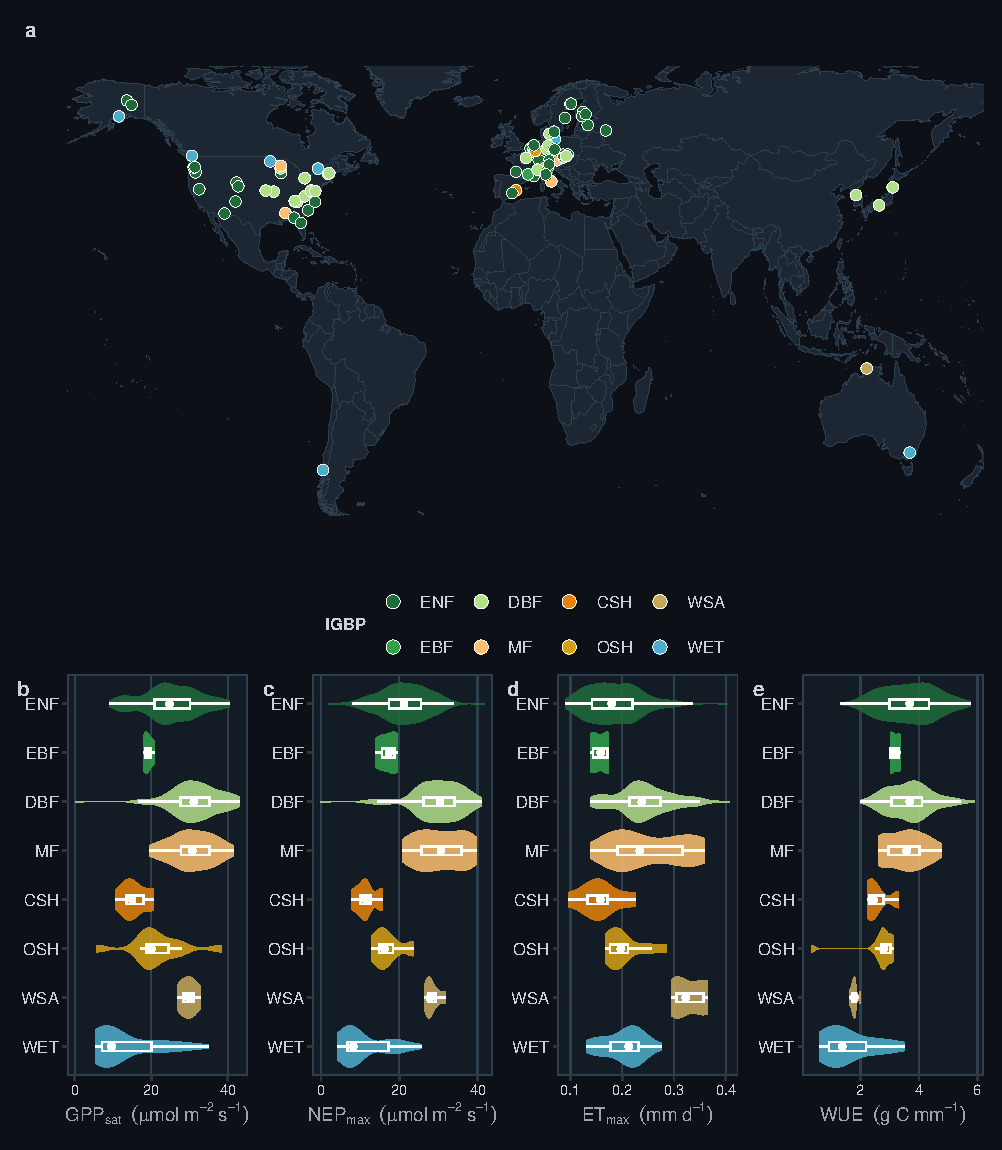
\includegraphics[width=\linewidth]{figures/fig1_site_map}\end{center}

\section*{Figure 2 --- Does disturbance reduce error? (M3 $\rightarrow$ M4)}
\begin{itemize}
  \item \textbf{Carbon fluxes: yes, consistently.} GPP$_{sat}$ significant in \textbf{12 of 12} configurations
        (median $-7.5$\,\%, range $-10.8$ to $-3.6$); NEP$_{max}$ \textbf{12 of 12} (median $-10.5$\,\%,
        range $-13.3$ to $-3.5$).
  \item \textbf{ET$_{max}$: a clean null.} \textbf{0 of 12} significant, median $+0.8$\,\%. Holds for every
        learner, window and CV structure.
  \item \textbf{WUE: intermediate.} 8 of 12 significant, median $-4.0$\,\% --- significant for XGBoost and
        LightGBM, not for random forest.
  \item \textbf{Learner matters little:} XGBoost 12/12, LightGBM 12/12, random forest 8/12 significant.
  \item \textbf{Cross-validation matters not at all:} \textbf{16 significant under LOO, 16 under repeated CV} ---
        identical counts, and the same tests.
  \item Roughly \textbf{60--78\,\% of sites} improve where the effect is significant; the effect is a shift in a
        broad distribution, not a uniform gain.
  \item \decide{report LOO in the main text and repeated CV in the supplement, or keep both here?}
  \item \decide{is WUE worth keeping given it is learner-dependent?}
\end{itemize}
\begin{center}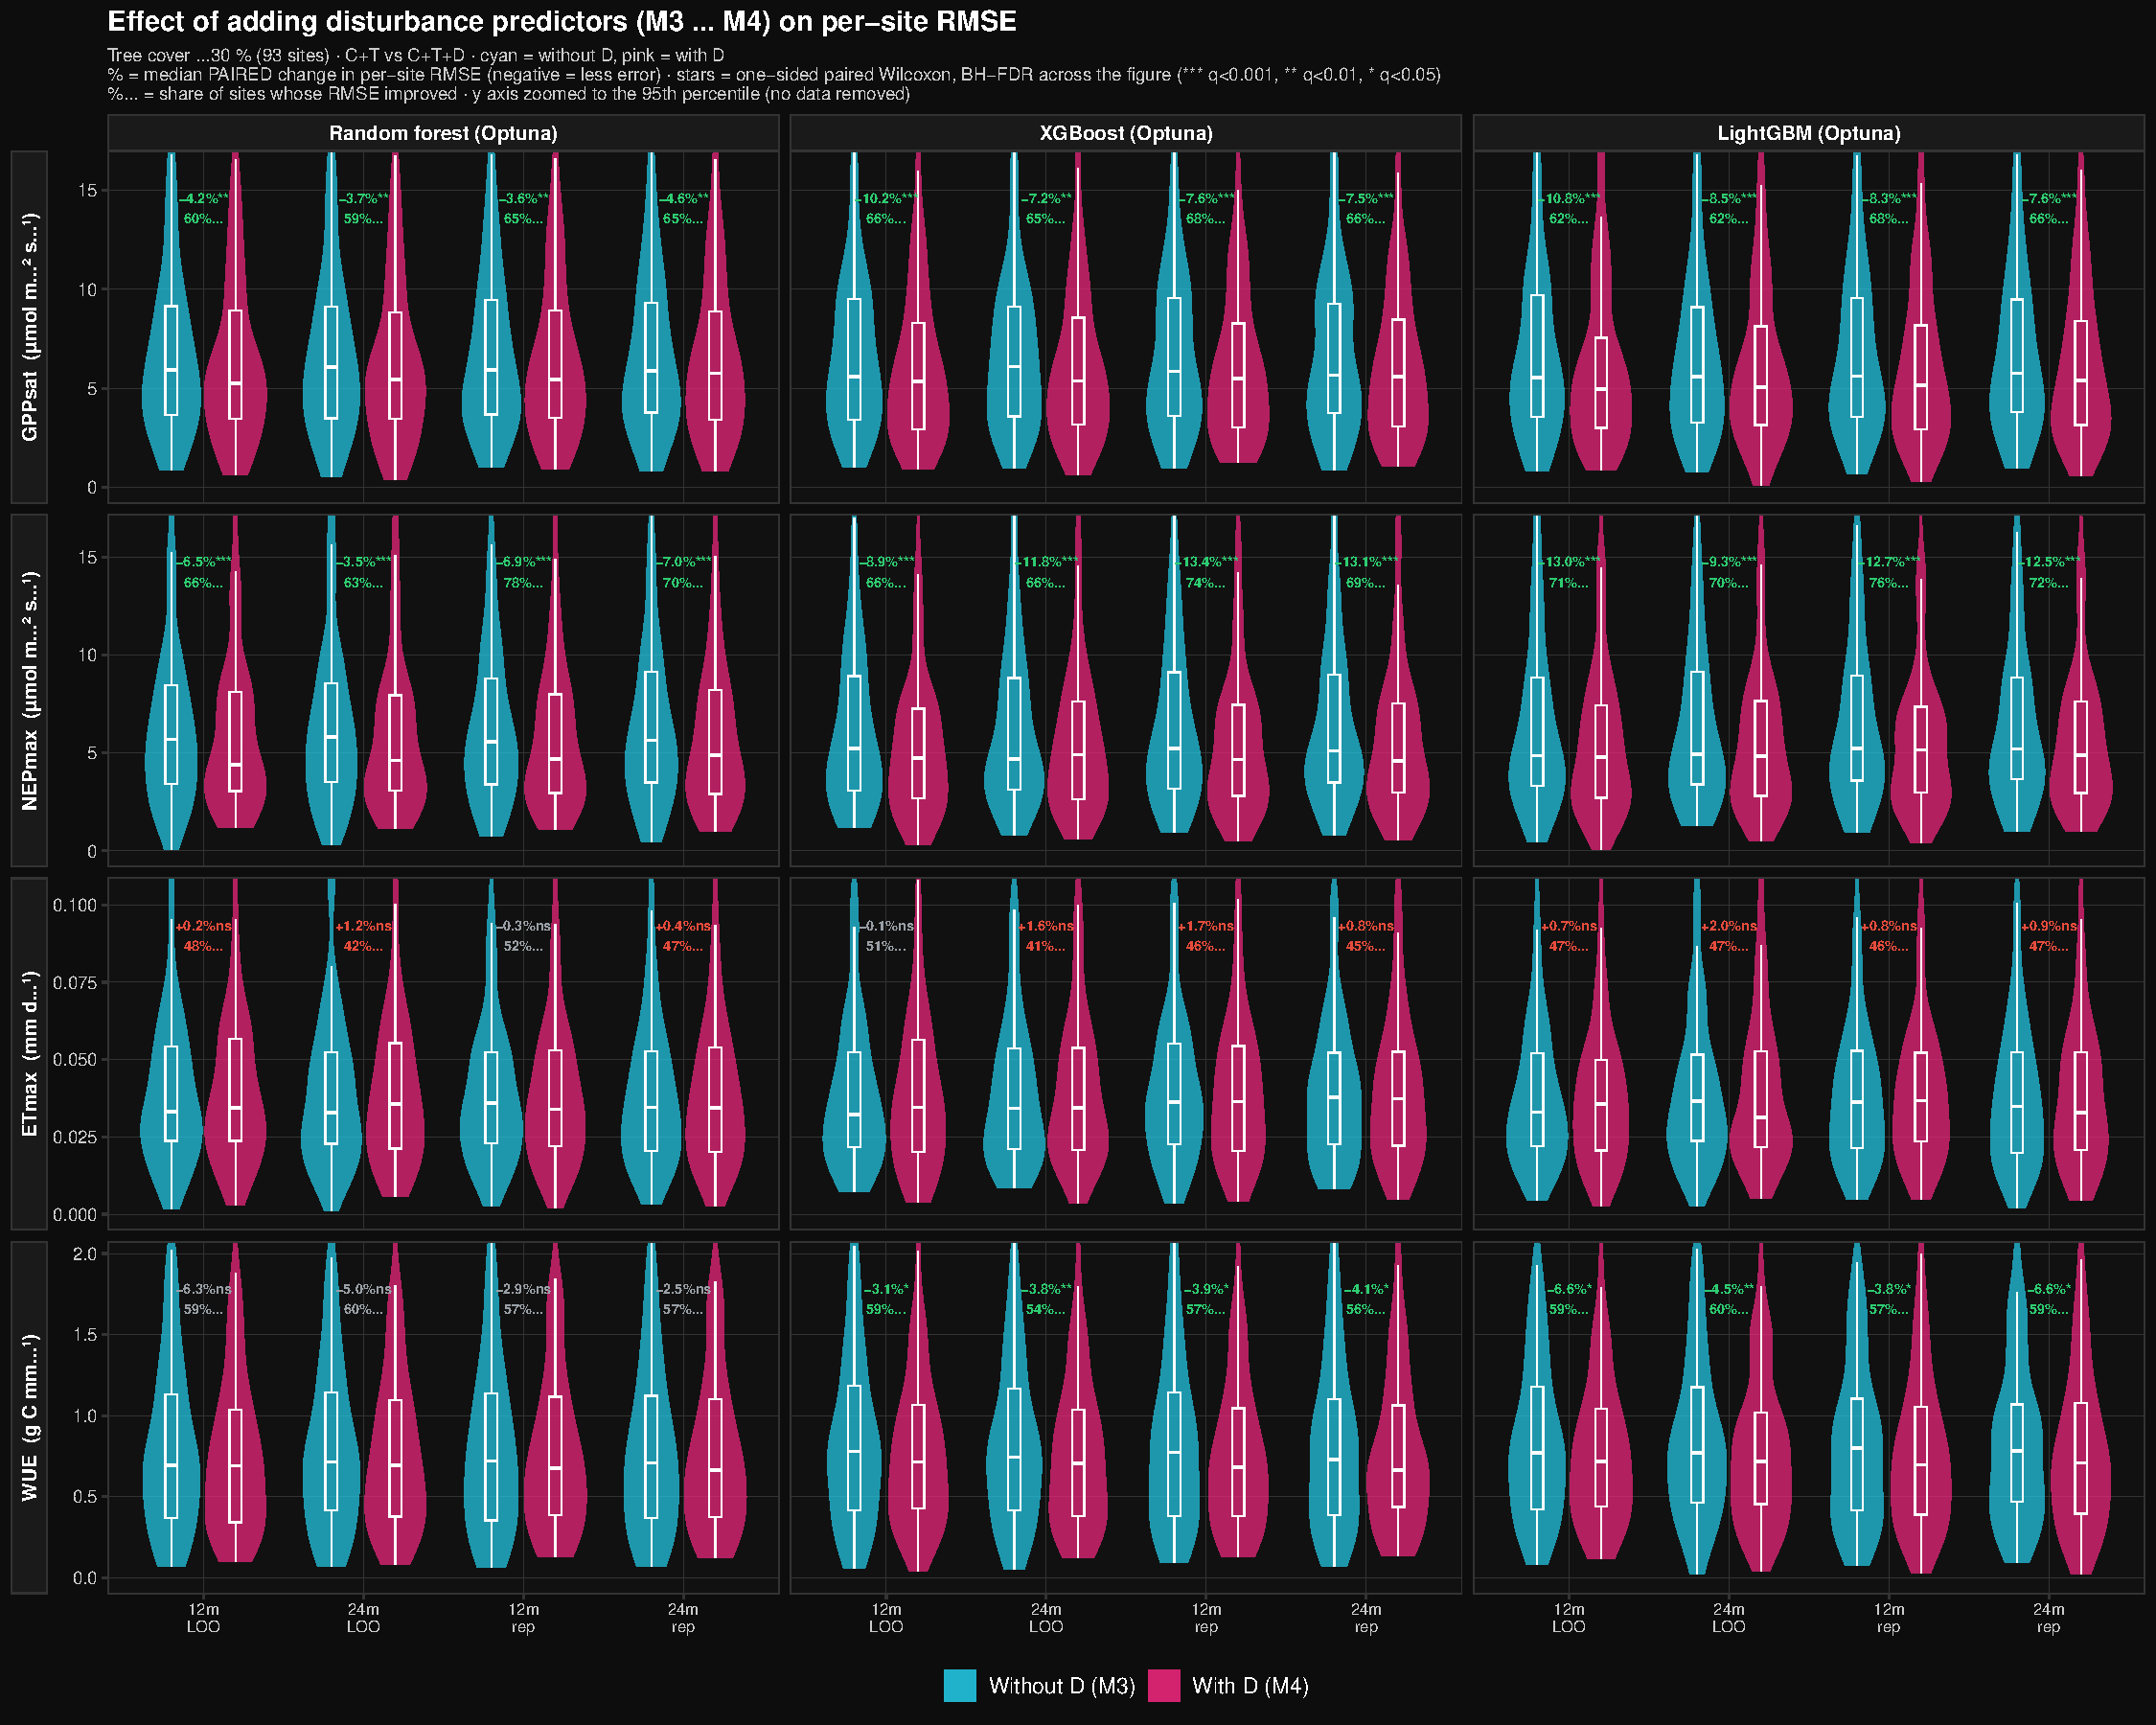
\includegraphics[width=\linewidth]{figures/fig2_disturbance_effect_M3M4}\end{center}

\section*{Figure 3 --- What the models actually use (per-site SHAP)}
\begin{itemize}
  \item Driver-group composition per site for M4, 12-month window. SHAP comes from full-data models, so it is
        identical under both CV structures.
  \item \textbf{Disturbance is consistently the second or third block}, never negligible where it matters:
        GPP$_{sat}$ 29\,\%, NEP$_{max}$ 31\,\%, WUE 38\,\%, ET$_{max}$ 13\,\% (mean across the three learners).
  \item \textbf{ET$_{max}$ is the outlier} --- climate takes 54\,\% and disturbance only 13\,\%, matching its
        null result in Figure 2. The two lines of evidence agree.
  \item Learners agree closely: the disturbance share spans only 27--31\,\% (GPP$_{sat}$) and 26--33\,\%
        (NEP$_{max}$) across the three.
  \item Strong \textbf{between-site spread} --- sites are ordered by disturbance share, and the left-hand sites
        draw almost nothing from the disturbance block.
  \item \decide{show the 24-month window as well, or keep 12-month only?}
\end{itemize}
\begin{center}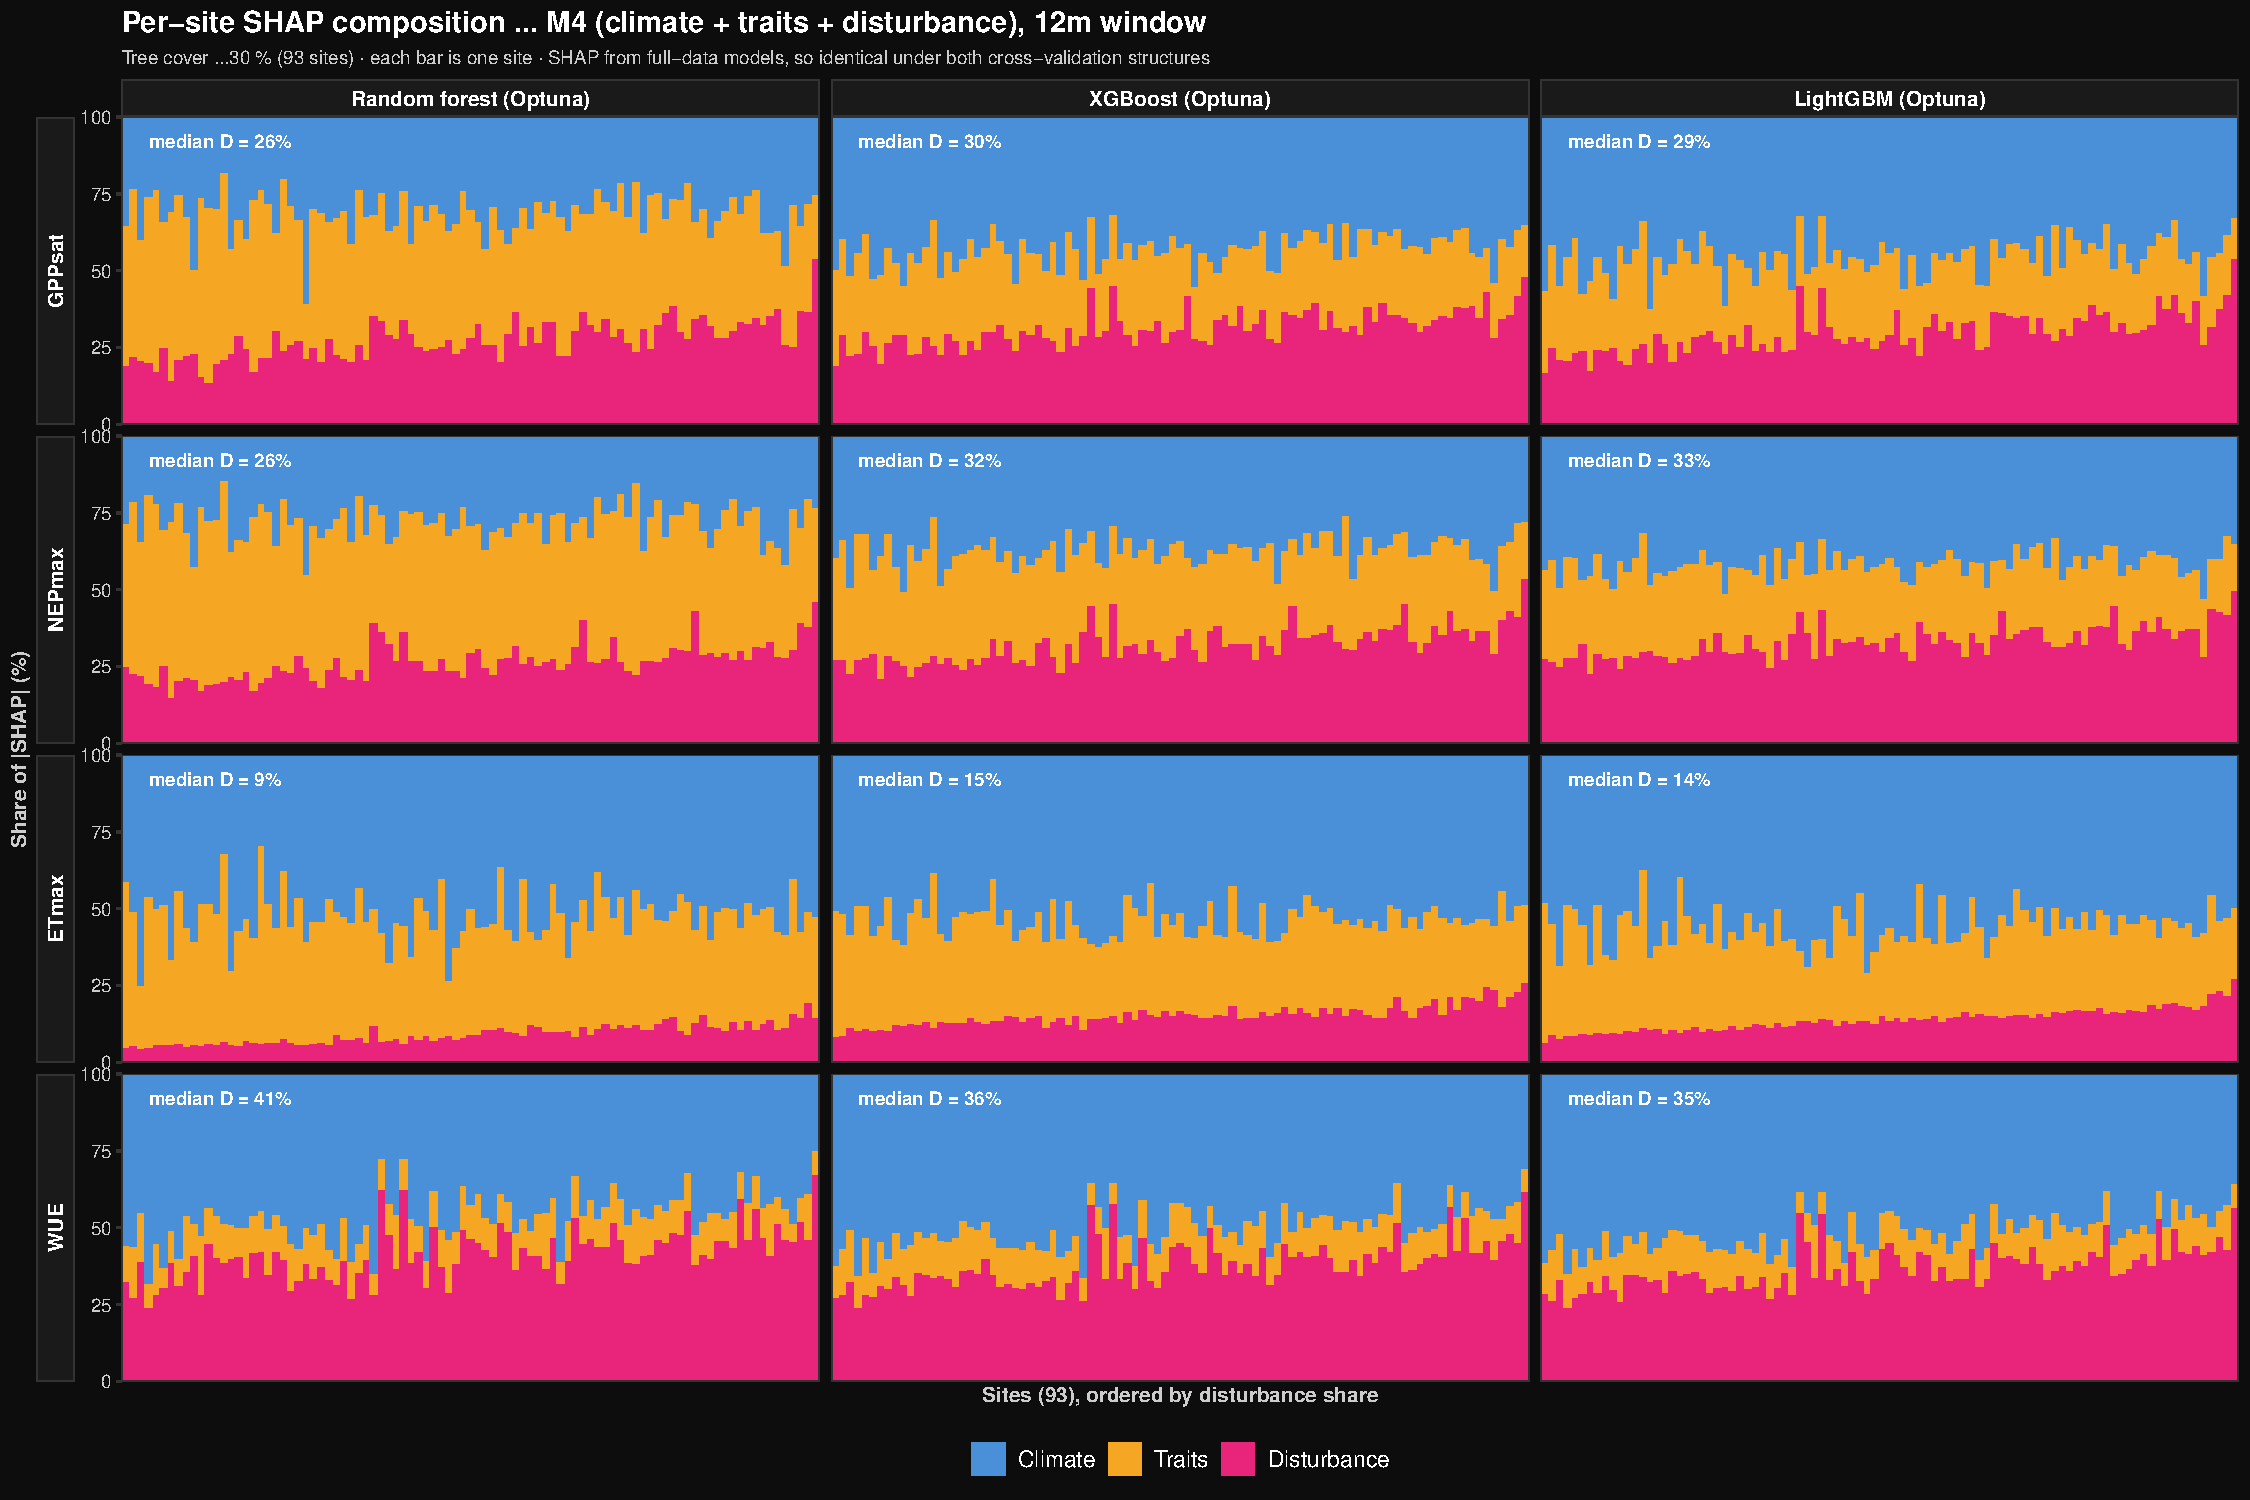
\includegraphics[width=\linewidth]{figures/fig3_site_shap_composition}\end{center}

\section*{Figure 4 --- Does the disturbance share scale with disturbance level?}
\begin{itemize}
  \item Disturbance share of $|$SHAP$|$ split by Low / Mid / High category, using tertile thresholds on three
        500\,m metrics (absolute mortality, relative mortality, relative disturbance).
  \item \textbf{Largely no.} Only \textbf{2 of 36} Kruskal--Wallis tests are significant after FDR correction,
        both for WUE. GPP$_{sat}$, NEP$_{max}$ and ET$_{max}$: 0 of 9 each.
  \item Models draw on the disturbance block at similar rates whether a site is heavily disturbed or not ---
        the block carries information about \emph{stand state}, not only about \emph{recent mortality events}.
  \item Consistent with the site-level heterogeneity in Figure 2: which sites benefit is not simply the
        most-disturbed ones.
  \item \decide{is this a main-text figure or a supplementary one? It is largely a negative result.}
  \item \decide{tertiles, equal-width or natural-breaks thresholds? All three exist; tertiles shown here.}
\end{itemize}
\begin{center}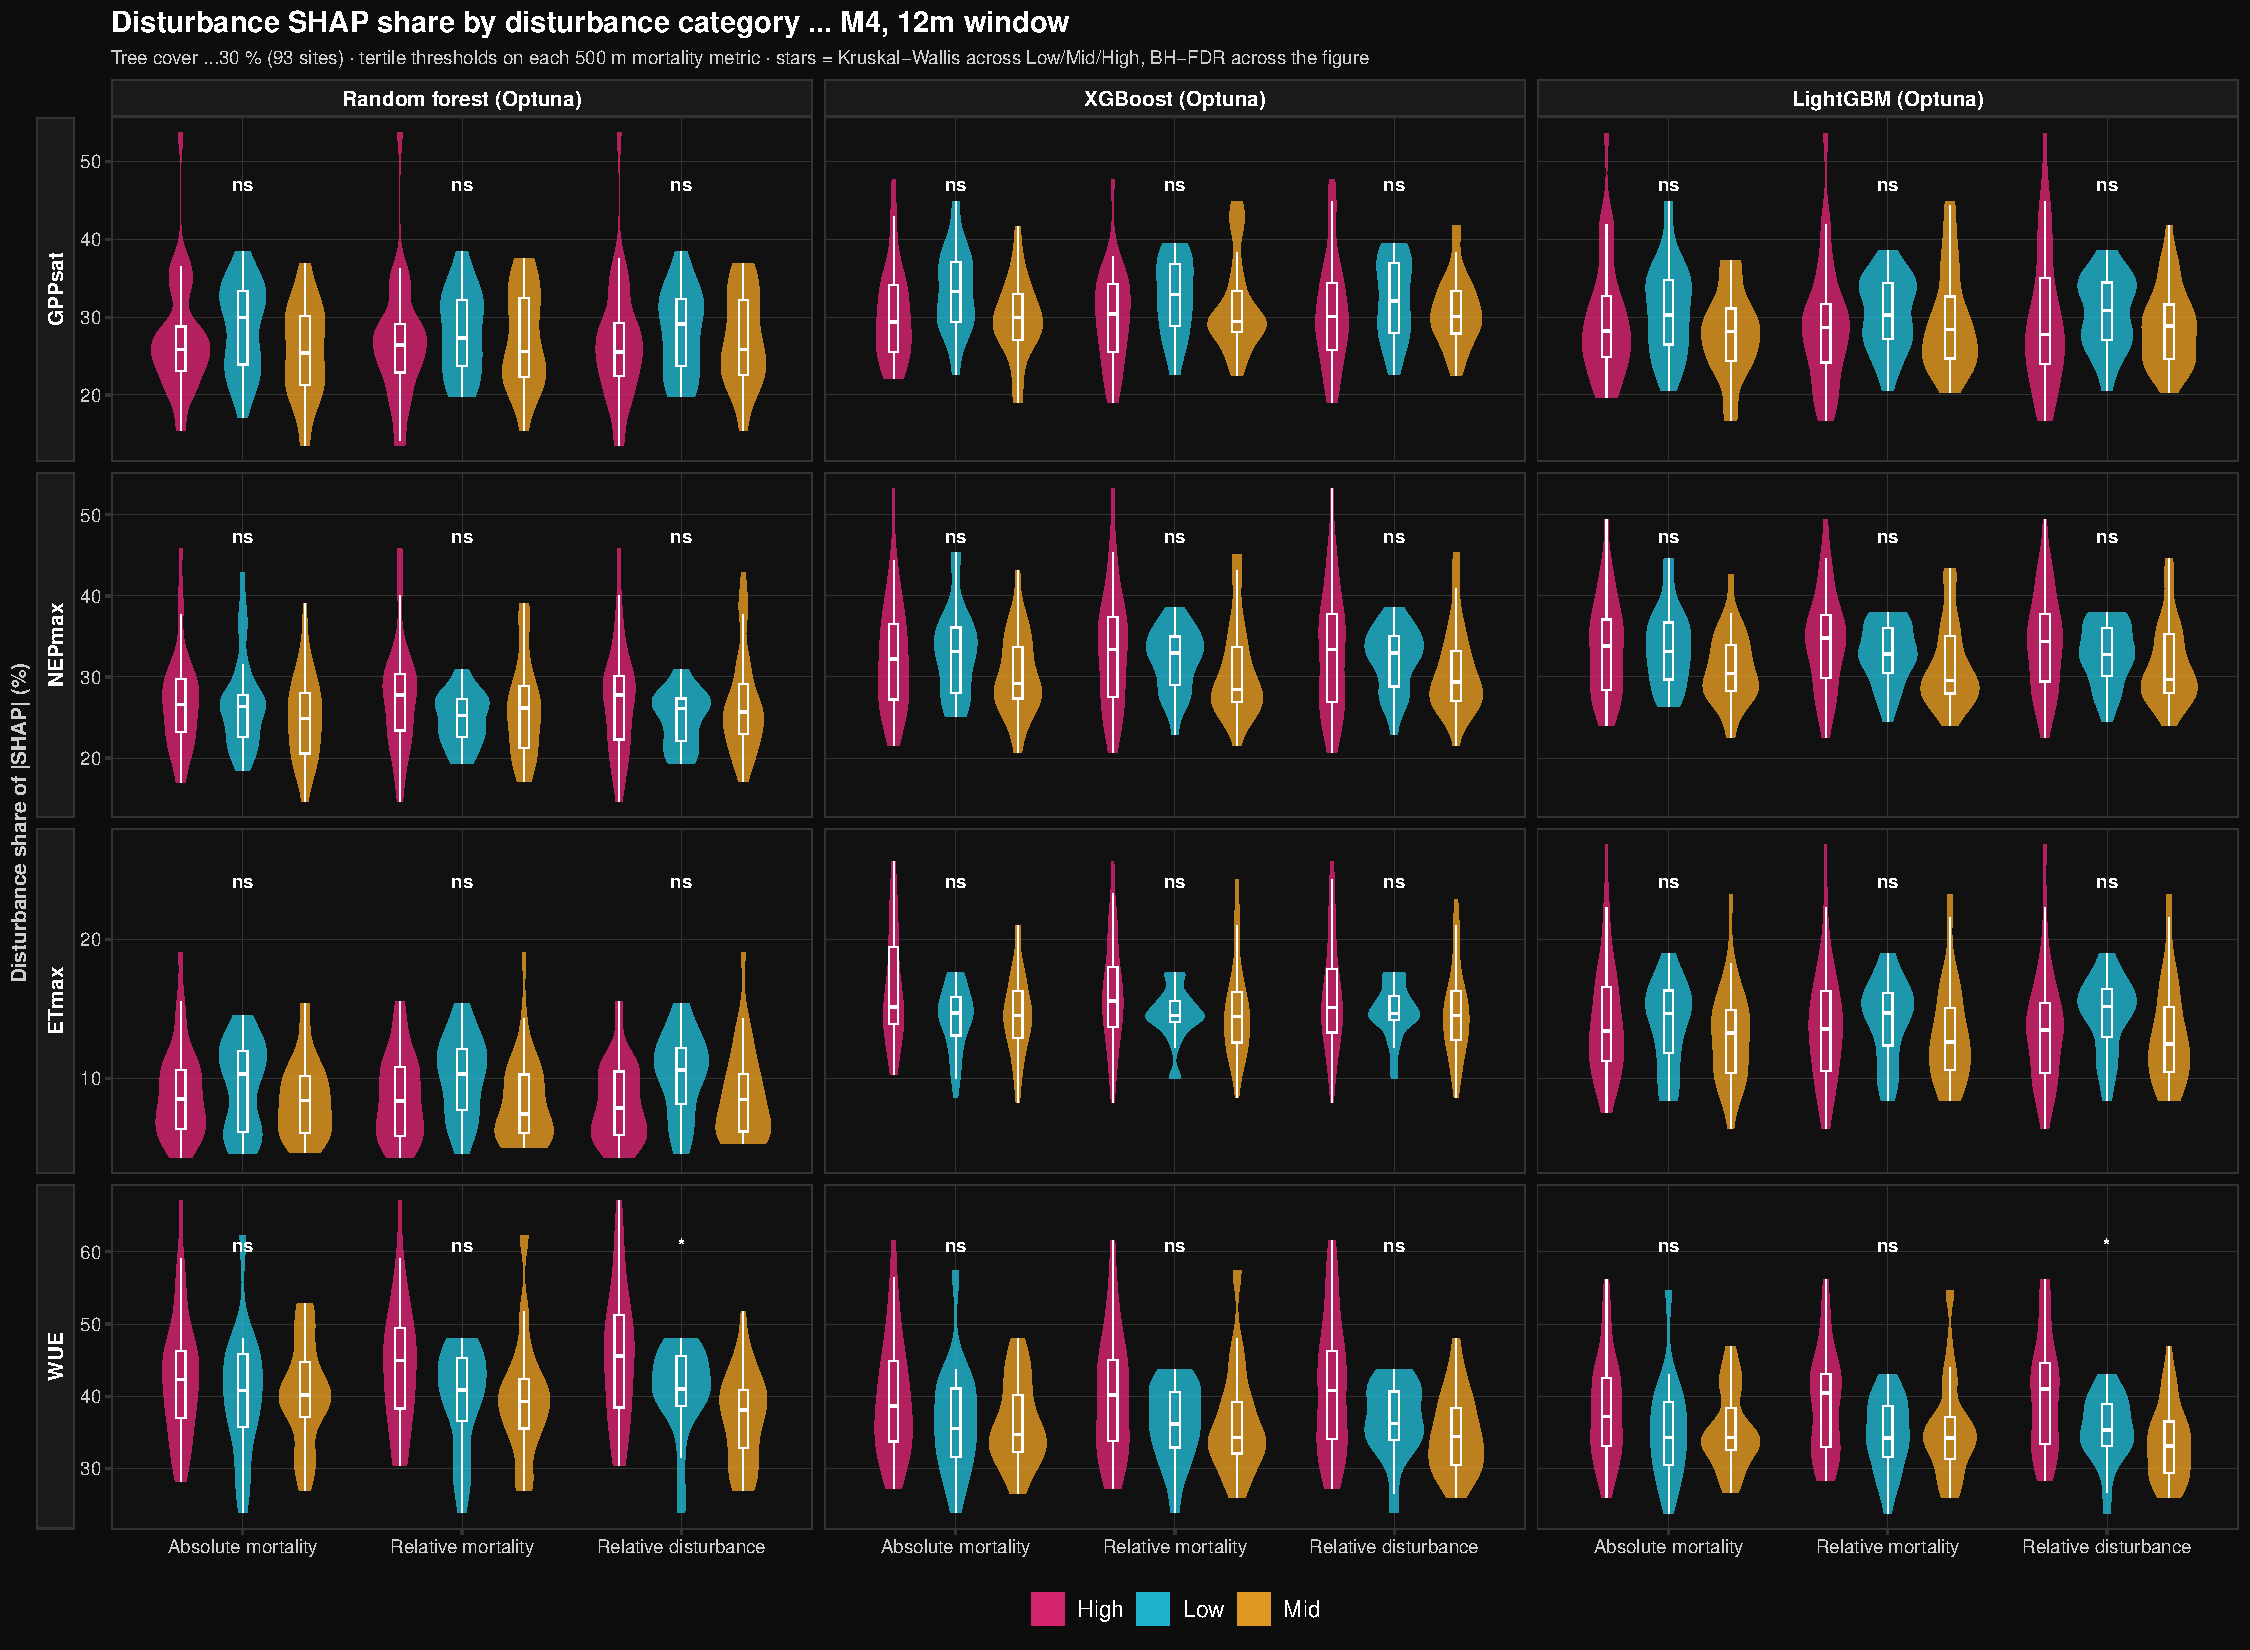
\includegraphics[width=\linewidth]{figures/fig4_grouped_disturbance_shap}\end{center}

\section*{Open decisions}
\begin{itemize}
  \item \textbf{Story.} Two candidate framings: (i) disturbance improves carbon-flux prediction but not water
        fluxes; (ii) the same, plus the memory result --- that the benefit largely disappears once the previous
        year's flux is known, so mortality data matter most where no flux tower exists. Framing (ii) is the
        stronger claim but needs M7/M8, which this draft excludes.
  \item \textbf{Dataset choice.} $\geq$30\,\% is shown. The disturbance effect is weaker on both the unfiltered
        network and the stricter $\geq$50\,\% subset, and does not scale with tree cover
        (Spearman $\rho = 0.04$, $p = 0.65$ at site level). Needs an \emph{a priori} justification in the text.
  \item \textbf{Learner to report.} XGBoost--Optuna suggested: best accuracy among configurations that impose no
        hand-set structure, and a mid-range disturbance effect rather than the largest.
  \item \textbf{uWUE.} Dropped here. It was the weakest and least consistent response throughout.
  \item \textbf{Figure style.} Dark background, matching the interactive report. Trivial to switch to white for
        submission.
\end{itemize}

\section*{Notes on the underlying results}
\begin{itemize}
  \item Statistics: one-sided paired Wilcoxon signed-rank on per-site RMSE, sites as the unit of replication,
        Benjamini--Hochberg FDR within each figure. Effect size is the \emph{median of the paired per-site
        differences}, not the difference of medians --- the two disagree in sign for some comparisons.
  \item Violin y-axes are zoomed to the 95th percentile for readability; no data are removed and all statistics
        use every site.
  \item \textbf{Known issue:} the random-forest Optuna SHAP table lost the names of the 14 trait variables whose
        names contain spaces, parentheses or slashes, placing $\sim$35\,\% of attribution in an unlabelled group.
        Group membership is unambiguous (14 unnamed + 7 named = the 21 traits the other learners show) and has
        been reassigned to Traits in Figures 3 and 4. The underlying extraction should still be fixed.
  \item Full results --- three datasets, nine learner configurations, both CV structures, all 24 model
        configurations --- are in the interactive report:
        \url{https://negin-katal.github.io/fluxVSmortality/v10/index.html}
\end{itemize}

\end{document}
